\begin{tikzpicture}
\pgfdeclareplotmark{cross} {
\pgfpathmoveto{\pgfpoint{-0.3\pgfplotmarksize}{\pgfplotmarksize}}
\pgfpathlineto{\pgfpoint{+0.3\pgfplotmarksize}{\pgfplotmarksize}}
\pgfpathlineto{\pgfpoint{+0.3\pgfplotmarksize}{0.3\pgfplotmarksize}}
\pgfpathlineto{\pgfpoint{+1\pgfplotmarksize}{0.3\pgfplotmarksize}}
\pgfpathlineto{\pgfpoint{+1\pgfplotmarksize}{-0.3\pgfplotmarksize}}
\pgfpathlineto{\pgfpoint{+0.3\pgfplotmarksize}{-0.3\pgfplotmarksize}}
\pgfpathlineto{\pgfpoint{+0.3\pgfplotmarksize}{-1.\pgfplotmarksize}}
\pgfpathlineto{\pgfpoint{-0.3\pgfplotmarksize}{-1.\pgfplotmarksize}}
\pgfpathlineto{\pgfpoint{-0.3\pgfplotmarksize}{-0.3\pgfplotmarksize}}
\pgfpathlineto{\pgfpoint{-1.\pgfplotmarksize}{-0.3\pgfplotmarksize}}
\pgfpathlineto{\pgfpoint{-1.\pgfplotmarksize}{0.3\pgfplotmarksize}}
\pgfpathlineto{\pgfpoint{-0.3\pgfplotmarksize}{0.3\pgfplotmarksize}}
\pgfpathclose
\pgfusepathqstroke
}
\pgfdeclareplotmark{cross*} {
\pgfpathmoveto{\pgfpoint{-0.3\pgfplotmarksize}{\pgfplotmarksize}}
\pgfpathlineto{\pgfpoint{+0.3\pgfplotmarksize}{\pgfplotmarksize}}
\pgfpathlineto{\pgfpoint{+0.3\pgfplotmarksize}{0.3\pgfplotmarksize}}
\pgfpathlineto{\pgfpoint{+1\pgfplotmarksize}{0.3\pgfplotmarksize}}
\pgfpathlineto{\pgfpoint{+1\pgfplotmarksize}{-0.3\pgfplotmarksize}}
\pgfpathlineto{\pgfpoint{+0.3\pgfplotmarksize}{-0.3\pgfplotmarksize}}
\pgfpathlineto{\pgfpoint{+0.3\pgfplotmarksize}{-1.\pgfplotmarksize}}
\pgfpathlineto{\pgfpoint{-0.3\pgfplotmarksize}{-1.\pgfplotmarksize}}
\pgfpathlineto{\pgfpoint{-0.3\pgfplotmarksize}{-0.3\pgfplotmarksize}}
\pgfpathlineto{\pgfpoint{-1.\pgfplotmarksize}{-0.3\pgfplotmarksize}}
\pgfpathlineto{\pgfpoint{-1.\pgfplotmarksize}{0.3\pgfplotmarksize}}
\pgfpathlineto{\pgfpoint{-0.3\pgfplotmarksize}{0.3\pgfplotmarksize}}
\pgfpathclose
\pgfusepathqfillstroke
}
\pgfdeclareplotmark{newstar} {
\pgfpathmoveto{\pgfqpoint{0pt}{\pgfplotmarksize}}
\pgfpathlineto{\pgfqpointpolar{44}{0.5\pgfplotmarksize}}
\pgfpathlineto{\pgfqpointpolar{18}{\pgfplotmarksize}}
\pgfpathlineto{\pgfqpointpolar{-20}{0.5\pgfplotmarksize}}
\pgfpathlineto{\pgfqpointpolar{-54}{\pgfplotmarksize}}
\pgfpathlineto{\pgfqpointpolar{-90}{0.5\pgfplotmarksize}}
\pgfpathlineto{\pgfqpointpolar{234}{\pgfplotmarksize}}
\pgfpathlineto{\pgfqpointpolar{198}{0.5\pgfplotmarksize}}
\pgfpathlineto{\pgfqpointpolar{162}{\pgfplotmarksize}}
\pgfpathlineto{\pgfqpointpolar{134}{0.5\pgfplotmarksize}}
\pgfpathclose
\pgfusepathqstroke
}
\pgfdeclareplotmark{newstar*} {
\pgfpathmoveto{\pgfqpoint{0pt}{\pgfplotmarksize}}
\pgfpathlineto{\pgfqpointpolar{44}{0.5\pgfplotmarksize}}
\pgfpathlineto{\pgfqpointpolar{18}{\pgfplotmarksize}}
\pgfpathlineto{\pgfqpointpolar{-20}{0.5\pgfplotmarksize}}
\pgfpathlineto{\pgfqpointpolar{-54}{\pgfplotmarksize}}
\pgfpathlineto{\pgfqpointpolar{-90}{0.5\pgfplotmarksize}}
\pgfpathlineto{\pgfqpointpolar{234}{\pgfplotmarksize}}
\pgfpathlineto{\pgfqpointpolar{198}{0.5\pgfplotmarksize}}
\pgfpathlineto{\pgfqpointpolar{162}{\pgfplotmarksize}}
\pgfpathlineto{\pgfqpointpolar{134}{0.5\pgfplotmarksize}}
\pgfpathclose
\pgfusepathqfillstroke
}
\definecolor{c}{rgb}{1,1,1};
\draw [color=c, fill=c] (0,0) rectangle (20,14.3108);
\draw [color=c, fill=c] (3.2,2.28972) rectangle (19,13.5952);
\definecolor{c}{rgb}{0,0,0};
\draw [c,line width=0.9] (3.2,2.28972) -- (3.2,13.5952) -- (19,13.5952) -- (19,2.28972) -- (3.2,2.28972);
\definecolor{c}{rgb}{0.325123,0.404902,0.834804};
\draw [color=c, fill=c] (3.2,2.28972) rectangle (6.53333,4.40951);
\definecolor{c}{rgb}{0.411887,0.487255,0.840686};
\draw [color=c, fill=c] (6.53333,2.28972) rectangle (9.86667,4.40951);
\definecolor{c}{rgb}{0.598284,0.651348,0.859804};
\draw [color=c, fill=c] (9.86667,2.28972) rectangle (12.3333,4.40951);
\definecolor{c}{rgb}{0.821814,0.835294,0.83652};
\draw [color=c, fill=c] (13.3333,2.28972) rectangle (16.5333,4.40951);
\definecolor{c}{rgb}{0.878922,0.873775,0.389461};
\draw [color=c, fill=c] (16.5333,2.28972) rectangle (19,4.40951);
\definecolor{c}{rgb}{0.411887,0.487255,0.840686};
\draw [color=c, fill=c] (3.2,4.40951) rectangle (6.53333,5.8227);
\draw [color=c, fill=c] (6.53333,4.40951) rectangle (9.86667,5.8227);
\definecolor{c}{rgb}{0.690686,0.726225,0.872549};
\draw [color=c, fill=c] (9.86667,4.40951) rectangle (12.3333,5.8227);
\definecolor{c}{rgb}{0.885417,0.895466,0.513726};
\draw [color=c, fill=c] (13.3333,4.40951) rectangle (16.5333,5.8227);
\definecolor{c}{rgb}{0.724265,0.203186,0.13125};
\draw [color=c, fill=c] (16.5333,4.40951) rectangle (19,5.8227);
\definecolor{c}{rgb}{0.411887,0.487255,0.840686};
\draw [color=c, fill=c] (3.2,5.8227) rectangle (6.53333,7.94248);
\definecolor{c}{rgb}{0.505882,0.576471,0.847059};
\draw [color=c, fill=c] (6.53333,5.8227) rectangle (9.86667,7.94248);
\definecolor{c}{rgb}{0.690686,0.726225,0.872549};
\draw [color=c, fill=c] (9.86667,5.8227) rectangle (12.3333,7.94248);
\definecolor{c}{rgb}{0.885417,0.895466,0.513726};
\draw [color=c, fill=c] (13.3333,5.8227) rectangle (16.5333,7.94248);
\definecolor{c}{rgb}{0.703676,0.0590686,0.115074};
\draw [color=c, fill=c] (16.5333,5.8227) rectangle (19,7.94248);
\definecolor{c}{rgb}{0.411887,0.487255,0.840686};
\draw [color=c, fill=c] (3.2,7.94248) rectangle (6.53333,13.5952);
\definecolor{c}{rgb}{0.505882,0.576471,0.847059};
\draw [color=c, fill=c] (6.53333,7.94248) rectangle (9.86667,13.5952);
\definecolor{c}{rgb}{0.690686,0.726225,0.872549};
\draw [color=c, fill=c] (9.86667,7.94248) rectangle (12.3333,13.5952);
\definecolor{c}{rgb}{0.883946,0.891054,0.654902};
\draw [color=c, fill=c] (13.3333,7.94248) rectangle (16.5333,13.5952);
\definecolor{c}{rgb}{0.703676,0.0590686,0.115074};
\draw [color=c, fill=c] (16.5333,7.94248) rectangle (19,13.5952);
\definecolor{c}{rgb}{0.187982,0.25351,0.88425};
\draw [color=c, fill=c] (19.1,2.28972) rectangle (19.99,2.855);
\definecolor{c}{rgb}{0.247185,0.324225,0.848071};
\draw [color=c, fill=c] (19.1,2.855) rectangle (19.99,3.42028);
\definecolor{c}{rgb}{0.325123,0.404902,0.834804};
\draw [color=c, fill=c] (19.1,3.42028) rectangle (19.99,3.98555);
\definecolor{c}{rgb}{0.411887,0.487255,0.840686};
\draw [color=c, fill=c] (19.1,3.98555) rectangle (19.99,4.55083);
\definecolor{c}{rgb}{0.505882,0.576471,0.847059};
\draw [color=c, fill=c] (19.1,4.55083) rectangle (19.99,5.1161);
\definecolor{c}{rgb}{0.598284,0.651348,0.859804};
\draw [color=c, fill=c] (19.1,5.1161) rectangle (19.99,5.68138);
\definecolor{c}{rgb}{0.690686,0.726225,0.872549};
\draw [color=c, fill=c] (19.1,5.68138) rectangle (19.99,6.24665);
\definecolor{c}{rgb}{0.761275,0.784314,0.865196};
\draw [color=c, fill=c] (19.1,6.24665) rectangle (19.99,6.81193);
\definecolor{c}{rgb}{0.821814,0.835294,0.83652};
\draw [color=c, fill=c] (19.1,6.81193) rectangle (19.99,7.37721);
\definecolor{c}{rgb}{0.882353,0.886275,0.807843};
\draw [color=c, fill=c] (19.1,7.37721) rectangle (19.99,7.94248);
\definecolor{c}{rgb}{0.883946,0.891054,0.654902};
\draw [color=c, fill=c] (19.1,7.94248) rectangle (19.99,8.50776);
\definecolor{c}{rgb}{0.885417,0.895466,0.513726};
\draw [color=c, fill=c] (19.1,8.50776) rectangle (19.99,9.07303);
\definecolor{c}{rgb}{0.878922,0.873775,0.389461};
\draw [color=c, fill=c] (19.1,9.07303) rectangle (19.99,9.63831);
\definecolor{c}{rgb}{0.86299,0.821201,0.298652};
\draw [color=c, fill=c] (19.1,9.63831) rectangle (19.99,10.2036);
\definecolor{c}{rgb}{0.847059,0.768627,0.207843};
\draw [color=c, fill=c] (19.1,10.2036) rectangle (19.99,10.7689);
\definecolor{c}{rgb}{0.813235,0.642157,0.188725};
\draw [color=c, fill=c] (19.1,10.7689) rectangle (19.99,11.3341);
\definecolor{c}{rgb}{0.776593,0.505147,0.168015};
\draw [color=c, fill=c] (19.1,11.3341) rectangle (19.99,11.8994);
\definecolor{c}{rgb}{0.746569,0.359314,0.148775};
\draw [color=c, fill=c] (19.1,11.8994) rectangle (19.99,12.4647);
\definecolor{c}{rgb}{0.724265,0.203186,0.13125};
\draw [color=c, fill=c] (19.1,12.4647) rectangle (19.99,13.03);
\definecolor{c}{rgb}{0.703676,0.0590686,0.115074};
\draw [color=c, fill=c] (19.1,13.03) rectangle (19.99,13.5952);
\definecolor{c}{rgb}{0,0,0};
\draw [c,line width=0.9] (19.99,2.28972) -- (19.99,13.5952);
\draw [c,line width=0.9] (19.516,2.28972) -- (19.99,2.28972);
\draw [c,line width=0.9] (19.516,4.16046) -- (19.99,4.16046);
\draw [c,line width=0.9] (19.516,6.03119) -- (19.99,6.03119);
\draw [c,line width=0.9] (19.516,7.90192) -- (19.99,7.90192);
\draw [c,line width=0.9] (19.516,9.77265) -- (19.99,9.77265);
\draw [c,line width=0.9] (19.516,11.6434) -- (19.99,11.6434);
\draw [c,line width=0.9] (19.516,13.5141) -- (19.99,13.5141);
\draw [c,line width=0.9] (19.516,13.5141) -- (19.99,13.5141);
\draw [anchor= west] (20.09,2.28972) node[scale=1.11327, color=c, rotate=0]{0};
\draw [anchor= west] (20.09,4.16046) node[scale=1.11327, color=c, rotate=0]{0.02};
\draw [anchor= west] (20.09,6.03119) node[scale=1.11327, color=c, rotate=0]{0.04};
\draw [anchor= west] (20.09,7.90192) node[scale=1.11327, color=c, rotate=0]{0.06};
\draw [anchor= west] (20.09,9.77265) node[scale=1.11327, color=c, rotate=0]{0.08};
\draw [anchor= west] (20.09,11.6434) node[scale=1.11327, color=c, rotate=0]{0.1};
\draw [anchor= west] (20.09,13.5141) node[scale=1.11327, color=c, rotate=0]{0.12};
\draw (4.86667,3.34962) node[scale=1.61424, color=c, rotate=1]{$\genfrac{}{}{0pt}{}{0.0142}{\pm 0.0002}$};
\draw (8.2,3.34962) node[scale=1.61424, color=c, rotate=1]{$\genfrac{}{}{0pt}{}{0.0184}{\pm 0.0005}$};
\draw (11.1,3.34962) node[scale=1.61424, color=c, rotate=1]{$\genfrac{}{}{0pt}{}{0.0328}{\pm 0.0005}$};
\draw (14.9333,3.34962) node[scale=1.61424, color=c, rotate=1]{$\genfrac{}{}{0pt}{}{0.0507}{\pm 0.0006}$};
\draw (17.7667,3.34962) node[scale=1.61424, color=c, rotate=1]{$\genfrac{}{}{0pt}{}{0.0749}{\pm 0.0008}$};
\draw (4.86667,5.1161) node[scale=1.61424, color=c, rotate=1]{$\genfrac{}{}{0pt}{}{0.0197}{\pm 0.0002}$};
\draw (8.2,5.1161) node[scale=1.61424, color=c, rotate=1]{$\genfrac{}{}{0pt}{}{0.0230}{\pm 0.0002}$};
\draw (11.1,5.1161) node[scale=1.61424, color=c, rotate=1]{$\genfrac{}{}{0pt}{}{0.0403}{\pm 0.0004}$};
\draw (14.9333,5.1161) node[scale=1.61424, color=c, rotate=1]{$\genfrac{}{}{0pt}{}{0.0671}{\pm 0.0005}$};
\draw (17.7667,5.1161) node[scale=1.61424, color=c, rotate=1]{$\genfrac{}{}{0pt}{}{0.1131}{\pm 0.0009}$};
\draw (4.86667,6.88259) node[scale=1.61424, color=c, rotate=1]{$\genfrac{}{}{0pt}{}{0.0203}{\pm 0.0003}$};
\draw (8.2,6.88259) node[scale=1.61424, color=c, rotate=1]{$\genfrac{}{}{0pt}{}{0.0247}{\pm 0.0004}$};
\draw (11.1,6.88259) node[scale=1.61424, color=c, rotate=1]{$\genfrac{}{}{0pt}{}{0.0408}{\pm 0.0006}$};
\draw (14.9333,6.88259) node[scale=1.61424, color=c, rotate=1]{$\genfrac{}{}{0pt}{}{0.0670}{\pm 0.0008}$};
\draw (17.7667,6.88259) node[scale=1.61424, color=c, rotate=1]{$\genfrac{}{}{0pt}{}{0.1209}{\pm 0.0015}$};
\draw (4.86667,10.7689) node[scale=1.61424, color=c, rotate=1]{$\genfrac{}{}{0pt}{}{0.0224}{\pm 0.0024}$};
\draw (8.2,10.7689) node[scale=1.61424, color=c, rotate=1]{$\genfrac{}{}{0pt}{}{0.0263}{\pm 0.0015}$};
\draw (11.1,10.7689) node[scale=1.61424, color=c, rotate=1]{$\genfrac{}{}{0pt}{}{0.0385}{\pm 0.0023}$};
\draw (14.9333,10.7689) node[scale=1.61424, color=c, rotate=1]{$\genfrac{}{}{0pt}{}{0.0637}{\pm 0.0029}$};
\draw (17.7667,10.7689) node[scale=1.61424, color=c, rotate=1]{$\genfrac{}{}{0pt}{}{0.1155}{\pm 0.0054}$};
\draw [c,line width=0.9] (3.2,2.28972) -- (19,2.28972);
\draw [anchor=north] (4.86667,2.12014) node[scale=0.723624, color=c, rotate=0]{[0.0 - 0.5]};
\draw [anchor=north] (8.2,2.12014) node[scale=0.723624, color=c, rotate=0]{[0.5 - 1.0]};
\draw [anchor=north] (11.1,2.12014) node[scale=0.723624, color=c, rotate=0]{[1.0 - 1.37]};
\draw [anchor=north] (14.9333,2.12014) node[scale=0.723624, color=c, rotate=0]{[1.52 - 2.0]};
\draw [anchor=north] (17.7667,2.12014) node[scale=0.723624, color=c, rotate=0]{[2.0 - 2.37]};
\draw [c,line width=0.9] (3.2,2.62889) -- (3.2,2.28972);
\draw [c,line width=0.9] (6.53333,2.62889) -- (6.53333,2.28972);
\draw [c,line width=0.9] (9.86667,2.62889) -- (9.86667,2.28972);
\draw [c,line width=0.9] (13.2,2.62889) -- (13.2,2.28972);
\draw [c,line width=0.9] (16.5333,2.62889) -- (16.5333,2.28972);
\draw [c,line width=0.9] (16.5333,2.62889) -- (16.5333,2.28972);
\draw [anchor= east] (19,1.16776) node[scale=1.11327, color=c, rotate=0]{$|\eta|_{  e}^{probe}$};
\draw [c,line width=0.9] (3.2,13.5952) -- (19,13.5952);
\draw [c,line width=0.9] (3.2,13.2561) -- (3.2,13.5952);
\draw [c,line width=0.9] (6.53333,13.2561) -- (6.53333,13.5952);
\draw [c,line width=0.9] (9.86667,13.2561) -- (9.86667,13.5952);
\draw [c,line width=0.9] (13.2,13.2561) -- (13.2,13.5952);
\draw [c,line width=0.9] (16.5333,13.2561) -- (16.5333,13.5952);
\draw [c,line width=0.9] (16.5333,13.2561) -- (16.5333,13.5952);
\draw [c,line width=0.9] (3.2,2.28972) -- (3.2,13.5952);
\draw [anchor= east] (2.963,3.34962) node[scale=0.723624, color=c, rotate=0]{[20 - 35] };
\draw [anchor= east] (2.963,5.1161) node[scale=0.723624, color=c, rotate=0]{[35 - 45] };
\draw [anchor= east] (2.963,6.88259) node[scale=0.723624, color=c, rotate=0]{[45 - 60] };
\draw [anchor= east] (2.963,10.7689) node[scale=0.723624, color=c, rotate=0]{[60 - 100]};
\draw [c,line width=0.9] (3.674,2.28972) -- (3.2,2.28972);
\draw [c,line width=0.9] (3.674,5.1161) -- (3.2,5.1161);
\draw [c,line width=0.9] (3.674,7.94248) -- (3.2,7.94248);
\draw [c,line width=0.9] (3.674,10.7689) -- (3.2,10.7689);
\draw [c,line width=0.9] (3.674,13.5952) -- (3.2,13.5952);
\draw [anchor= east] (1.632,13.5952) node[scale=1.11327, color=c, rotate=90]{$p_{T,  e}^{probe}  [GeV]$};
\draw [c,line width=0.9] (19,2.28972) -- (19,13.5952);
\draw [c,line width=0.9] (18.526,2.28972) -- (19,2.28972);
\draw [c,line width=0.9] (18.526,5.1161) -- (19,5.1161);
\draw [c,line width=0.9] (18.526,7.94248) -- (19,7.94248);
\draw [c,line width=0.9] (18.526,10.7689) -- (19,10.7689);
\draw [c,line width=0.9] (18.526,13.5952) -- (19,13.5952);
\end{tikzpicture}
